
\formulasheettitle{Synchronous Generator Model}%
{Formula sheet for the $xy0$ machine model}
\begin{noteBox}
	\textbf{Notation.} Subscripts $S$, $E$, $DX$, and $DY$ denote the stator,
	excitation winding, and the damper windings on the $x$- and $y$-axes.
	The dot denotes a time derivative, e.g. $\dot\psi=\diff\psi/\diff t$.
	The symbols $x$ and $y$ correspond to the rotating machine axes used in the
	source model.
\end{noteBox}

\begin{formulaBox}{Clarke transformation: three-phase to $xy0$}
	\begin{align}
		u_0   &= \frac{u_1+u_2+u_3}{3}
		= R_0 i_0 + L_0\dot i_0, \\
		u_{SXS} &= \frac{2u_1-(u_2+u_3)}{3}, \\
		u_{SYS} &= \frac{u_2-u_3}{\sqrt{3}}.
	\end{align}
	The stationary components are rotated through the electrical angle $\alpha$:
	\begin{align}
		u_{SX} &= u_{SXS}\cos\alpha + u_{SYS}\sin\alpha, \\
		u_{SY} &= u_{SYS}\cos\alpha - u_{SXS}\sin\alpha.
	\end{align}
\end{formulaBox}

\begin{formulaBox}{Electrical equations in the rotating reference frame}
	\begin{align}
		u_{SX} &= R_S i_{SX}+\dot\psi_{SX}-p\omega\psi_{SY}, \\
		g u_E  &= g^2\frac{2}{3}R_E i_E+\dot\psi_E, \\
		0      &= R_{DX}i_{DX}+\dot\psi_{DX}, \\
		u_{SY} &= R_S i_{SY}+\dot\psi_{SY}+p\omega\psi_{SX}, \\
		0      &= R_{DY}i_{DY}+\dot\psi_{DY}.
	\end{align}
\end{formulaBox}

\newpage
\thispagestyle{scrheadings}

\begin{formulaBox}{Flux linkages and current components}
	The common magnetizing flux linkages are
	\begin{align}
		\psi_{hX}
		&= \psi_{SX}-L_S i_{SX}
		= \psi_{DX}-L_{DX}i_{DX}
		= \psi_E-L_E\frac{i_E}{g}, \\
		\psi_{hY}
		&= \psi_{SY}-L_S i_{SY}
		= \psi_{DY}-L_{DY}i_{DY}.
	\end{align}
	The associated magnetizing currents are
	\begin{align}
		i_{\mu X}=f(\psi_{hX}) &= i_{SX}+i_{DX}+\frac{i_E}{g}, \\
		i_{\mu Y}=f(\psi_{hY}) &= i_{SY}+i_{DY}.
	\end{align}
	
	For the nonlinear magnetization characteristic shown in the source model,
	\begin{equation}
		i_\mu(\psi)=i_{\mu N}
		\left[
		0.9\frac{\psi}{\psi_N}
		+0.1\left(\frac{\psi}{\psi_N}\right)^7
		\right].
	\end{equation}
\end{formulaBox}

\begin{formulaBox}{Mechanical equations}
	\begin{align}
		M &= M_{RBG}-M_i, \\
		M_i &= \frac{3}{2}\,p\left(i_{SY}\psi_{hX}-i_{SX}\psi_{hY}\right), \\
		\alpha &= p\int \omega\,\diff t, \\
		M_{RBG} &= M_{\mathrm{Reibung}}\,\sign(n).
	\end{align}
	Here, $p$ is the number of pole pairs and $n$ is the mechanical speed.
\end{formulaBox}

\begin{formulaBox}{Inverse transformation: $xy0$ to three-phase}
	First rotate from the machine frame back to stationary coordinates:
	\begin{align}
		i_{SXS} &= i_{SX}\cos\alpha-i_{SY}\sin\alpha, \\
		i_{SYS} &= i_{SX}\sin\alpha+i_{SY}\cos\alpha.
	\end{align}
	Then recover the phase currents:
	\begin{align}
		i_1 &= i_{SXS}+i_0, \\
		i_2 &= \frac{-i_{SXS}+\sqrt{3}\,i_{SYS}}{2}+i_0, \\
		i_3 &= \frac{-i_{SXS}-\sqrt{3}\,i_{SYS}}{2}+i_0.
	\end{align}
\end{formulaBox}

\begin{noteBox}
	\textbf{Default model simplifications (if not otherwise supported by the parameter line):}
	\[
	\frac{i_E}{g}=i_E',\qquad
	L_E=L_S,\quad L_0=L_S,\quad L_{DX}=L_S,\quad L_{DY}=L_S,
	\]
	\[
	R_0=R_S,\qquad R_{DX}=R_D,\qquad R_{DY}=R_D.
	\]
\end{noteBox}

%\newpage
\thispagestyle{scrheadings}

\begin{formulaBox}{Constant machine parameters}
	The rated input data used for the \SI{400}{\mega\watt} synchronous generator are
	\begin{align}
		U_{N,\mathrm{verkettet}}&=\SI{20}{\kilo\volt}, &
		I_N&=\SI{14.434}{\kilo\ampere}, &
		P_{EL}&=\SI{400}{\mega\watt},\\
		f_N&=\SI{50}{\hertz}, &
		K_C&=0.5, &
		p&=2,\\
		U_{E0}&=\SI{600}{\volt}, &
		I_{E0}&=\SI{2000}{\ampere}, &
		\mathrm{Streuung}&=0.05,\\
		r_{cu}&=0.001, &
		r_{bg}&=0.001, &
		\mathrm{Schenkelpolfaktor}&=1,\\
		\mathrm{Daempferfaktor}&=1. &&&
	\end{align}
	
	The apparent power and power factor obtained from the rated voltage and current
	are
	\begin{align}
		S_N
		&=\sqrt{3}\,U_{N,\mathrm{verkettet}}I_N\\
		&=\sqrt{3}\cdot\SI{20}{\kilo\volt}
		\cdot\SI{14.434}{\kilo\ampere}
		=\SI{500.008}{\mega\volt\ampere}
		\approx\SI{500}{\mega\volt\ampere},\\
		\cos\varphi_N
		&=\frac{P_{EL}}{S_N}
		=\frac{\SI{400}{\mega\watt}}
		{\SI{500.008}{\mega\volt\ampere}}
		=0.799987\approx0.8.
	\end{align}
	
	The constant machine parameters are calculated from
	\begin{align}
		U_N &= \frac{U_{N,\mathrm{verkettet}}}{\sqrt{3}}, &
		Z_N &= \frac{U_N}{I_N}, \\
		\omega_{EL} &= 2\pi f_N, &
		R_S &= Z_N\,r_{cu}, \\
		L_S &= \frac{\mathrm{Streuung}\,Z_N}{K_C\omega_{EL}}, &
		\Psi_N &= \frac{\sqrt{2}\,U_N}{\omega_{EL}}, \\
		g &= \frac{I_{E0}(1-\mathrm{Streuung})}
		{K_C\sqrt{2}\,I_N}, &
		R_D &= \frac{R_S}{\mathrm{Daempferfaktor}}, \\
		I_{MNX} &= \frac{I_{E0}}{g}, &
		I_{MNY} &= \frac{I_{MNX}}{\mathrm{Schenkelpolfaktor}}, \\
		M_N &= \frac{pP_{EL}(1-r_{bg}-r_{cu})}{\omega_{EL}}. &&
	\end{align}
	
	Inserting the rated data gives
	\begin{align}
		U_N
		&=\frac{\SI{20}{\kilo\volt}}{\sqrt{3}}
		=\boxed{\SI{11.5470}{\kilo\volt}},\\
		Z_N
		&=\frac{\SI{11.5470}{\kilo\volt}}
		{\SI{14.434}{\kilo\ampere}}
		=\boxed{\SI{0.799987}{\ohm}},\\
		\omega_{EL}
		&=2\pi\cdot\SI{50}{\hertz}
		=\boxed{\SI{314.159}{\radian\per\second}},\\
		R_S
		&=\SI{0.799987}{\ohm}\cdot0.001
		=\boxed{\SI{7.99987e-4}{\ohm}},\\
		L_S
		&=\frac{0.05\cdot\SI{0.799987}{\ohm}}
		{0.5\cdot\SI{314.159}{\radian\per\second}}
		=\boxed{\SI{2.54644e-4}{\henry}},\\
		\Psi_N
		&=\frac{\sqrt{2}\cdot\SI{11.5470}{\kilo\volt}}
		{\SI{314.159}{\radian\per\second}}
		=\boxed{\SI{51.9798}{\weber}}.
	\end{align}
	
	For the excitation-current transformation,
	\begin{align}
		g
		&=\frac{\SI{2000}{\ampere}(1-0.05)}
		{0.5\sqrt{2}\cdot\SI{14.434}{\kilo\ampere}}
		=\boxed{0.186158},\\
		I_{MNX}
		&=\frac{\SI{2000}{\ampere}}{0.186158}
		=\boxed{\SI{10.7436}{\kilo\ampere}},\\
		I_{MNY}
		&=\frac{\SI{10.7436}{\kilo\ampere}}{1}
		=\boxed{\SI{10.7436}{\kilo\ampere}}.
	\end{align}
	
	Because \(\mathrm{Daempferfaktor}=1\), the damper resistance becomes
	\begin{equation}
		R_D=\frac{R_S}{1}
		=\boxed{\SI{7.99987e-4}{\ohm}}.
	\end{equation}
	
	The rated electromagnetic torque, including the specified relative friction
	and copper losses, is
	\begin{align}
		M_N
		&=\frac{2\cdot\SI{400}{\mega\watt}
			(1-0.001-0.001)}
		{\SI{314.159}{\radian\per\second}}\\
		&=\boxed{\SI{2.54139e6}{\newton\metre}}.
	\end{align}
	
	The excitation-winding resistance and its resistance referred to the stator side
	equation are
	\begin{align}
		R_E
		&=\frac{U_{E0}}{I_{E0}}
		=\frac{\SI{600}{\volt}}{\SI{2000}{\ampere}}
		=\boxed{\SI{0.300000}{\ohm}},\\
		R_E'
		&=g^2\frac{2}{3}R_E
		=(0.186158)^2\frac{2}{3}\cdot\SI{0.3}{\ohm}
		=\boxed{\SI{6.93097e-3}{\ohm}},\\
		U_{E0}'
		&=gU_{E0}
		=0.186158\cdot\SI{600}{\volt}
		=\boxed{\SI{111.695}{\volt}}.
	\end{align}
	
	For \(p=2\), the synchronous mechanical speed is
	\begin{align}
		n_N&=\frac{60f_N}{p}
		=\boxed{\SI{1500}{\rpm}}, &
		\omega_{mN}&=\frac{\omega_{EL}}{p}
		=\boxed{\SI{157.080}{\radian\per\second}}.
	\end{align}
	
\end{formulaBox}

\begin{noteBox}
	\textbf{Interpretation of \(\Psi_N\).}
	The value \(\Psi_N=\SI{51.9798}{\weber}\) is the rated peak stator flux
	linkage in volt-seconds, not the physical air-gap flux in webers per pole. A
	physical flux value would additionally require the effective number of stator
	turns and the winding factor.
\end{noteBox}

\begin{formulaBox}{Parameter definitions}
	\renewcommand{\arraystretch}{\formulaTableStretch}
	\begin{tabularx}{\textwidth}{>{\bfseries\(}l<{\)} X}
		\toprule
		\text{Symbol} & \textbf{Meaning} \\
		\midrule
		\mathrm{Streuung} & Leakage factor \\
		\mathrm{Daempferfaktor} & Damping factor \\
		\mathrm{Schenkelpolfaktor} & Salient-pole factor \\
		r_{bg} & Friction-loss factor \\
		r_{cu} & Copper-loss (resistance) factor \\
		p & Number of pole pairs \\
		K_C & Model scaling or correction factor \\
		U_{N,\mathrm{verkettet}} & Rated line-to-line RMS voltage \\
		U_N,\ I_N,\ Z_N & Rated phase voltage, rated current, and base impedance \\
		f_N,\ \omega_{EL} & Rated electrical frequency and angular frequency \\
		I_{E0} & Reference excitation current \\
		P_{EL} & Electrical power \\
		\bottomrule
	\end{tabularx}
\end{formulaBox}

\begin{widefigure}{Synchronous machine schematic model}{schematic111}
	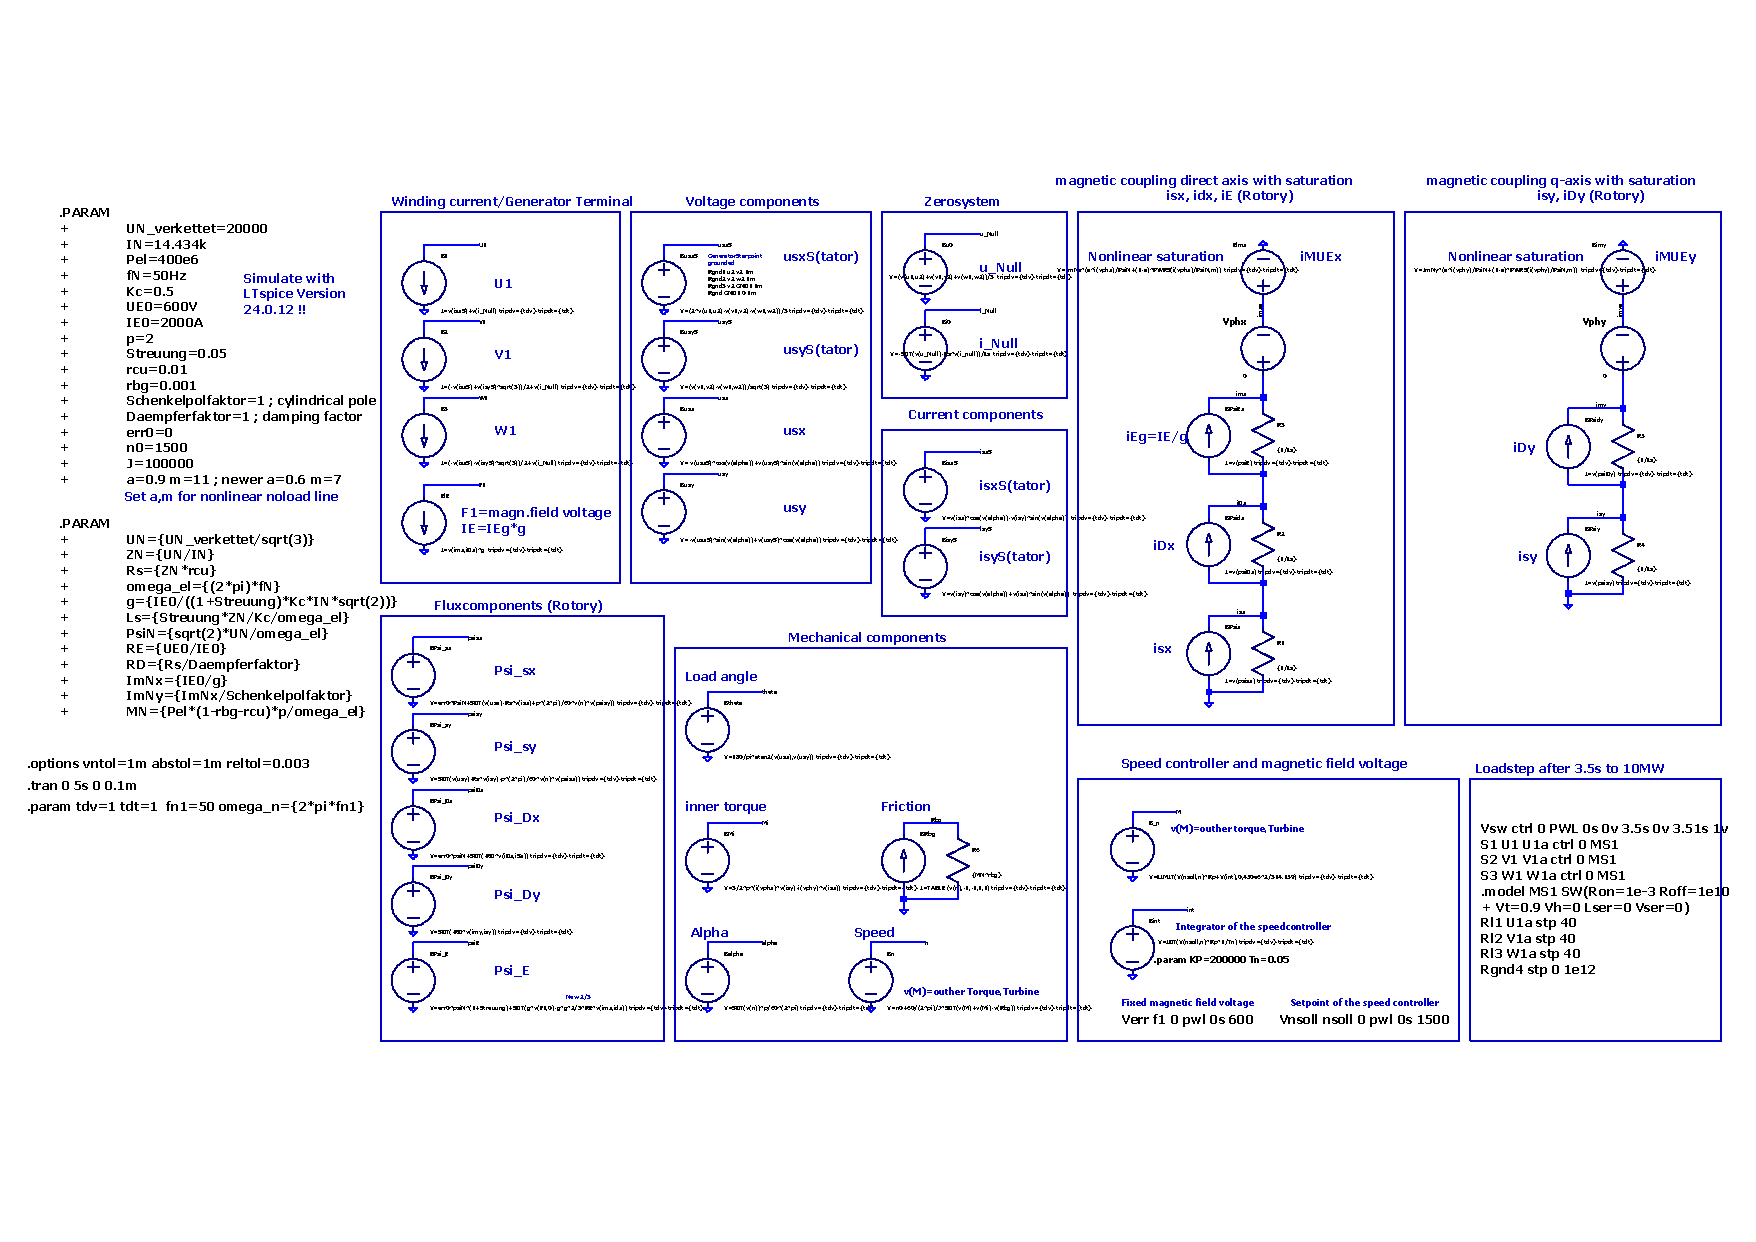
\includegraphics[width=1.5\textwidth]{figures/Synchronous_generator_model.pdf}
\end{widefigure}

%\begin{figure}[H]
%	\centering
%	\includegraphics[width=0.99\textwidth]{figures/Transformer_and_shunt_reactor_AC_Schematic}
%	\caption{Schematic for the Transformer and shunt reactor circuit.}
%	\label{fig:Transformer_and_shunt_reactor_AC_Schematic}
%\end{figure}

\begin{lstlisting}[style=LTspice,caption={Behavioral implementation of a synchronous generator.},label={lst:synchronous generator}]
1 * NOTE: idt() = integration function
2 .SUBCKT Block1_fixe_Drehzahl U1 V1 W1 F1 M n GND1
3 + PARAMS:
4 + UN_verkettet=20000
5 + IN=14.434k
6 + Pel=400e6 ;UN_verkettet*IN*sqrt(3)*cosphi of 0.8
7 + fn=50
8 + Kc=0.5
9 + UE0=600V ; Power of exciter = 0.25-5% * SN machine (smaller values for higher SN)
10 + IE0=2000A
11 + p=2
12 + Streuung=0.05 ;
13 + rcu=0.001
14 + rbg=0.001
15 + Schenkelpolfaktor=1 ;(1=cylindrical pole 0.5=Salient pole)
16 + Daempferfaktor=1
17 + err0=0
18 + RE_factor=0.6666
19 + n0=1500
20 + n1={n0} ;starts with 1500U/min
21 + alpha_0=0
22 + a=0.9 ; Parameter for nonlinear noload line (should be about 0.6-0.9)
23 + m=7
24 .PARAM
25 + a1={a}; Saturation parameter d-axis
26 + m1={m}; Saturation parameter d-axis
27 + a2={a1}; Saturation parameter q-axis
28 + m2={m1}; Saturation parameter q-axis
29 + UN={UN_verkettet/sqrt(3)}
30 + ZN={UN/IN}
31 + Rs={ZN*rcu}
32 + omega_el={(2*pi)*fN}
33 + Ls={Streuung*ZN/Kc/omega_el}
34 + PsiN={sqrt(2)*UN/omega_el}
35 + RE={UE0/IE0}
36 + RD={Rs/Daempferfaktor}
37 + RDx={RD} ; can be overwritten by setting this parameters on modelline
38 + RDy={RD} ; can be overwritten by setting this parameters on modelline
39 + LDx={Ls} ; can be overwritten by setting this parameters on modelline
40 + LDy={Ls} ; can be overwritten by setting this parameters on modelline
41 + LE={Ls} ; can be overwritten by setting this parameters on modelline
42 + R0={Rs} ; can be overwritten by setting this parameters on modelline
43 + L0={Ls} ; can be overwritten by setting this parameters on modelline (X0 is 0.03-0.1 p.u)
44 + Lsd={Ls}
45 + Lsq={Ls}
46 + XD={UN/IN/Kc}
47 + XQ={XD*Schenkelpolfaktor}
48 + g={UE0/(UN*sqrt(2)*RE/(XD-omega_el*Lsd))} ; updated formula for g parameter
49 + g1={UE0/(UN*sqrt(2)*RE/(XQ-omega_el*Lsq))} ; updated formula for salient pole machine
50 + ImNx={IE0/g} ; d-axis magnetizing current
51 + ImNy={IE0/g1} ;q-axis magnetizing current
52 + MN={Pel*(1-rbg-rcu)*p/omega_el}
53 *
54 * currents of windings
55 G1 U1 U2 VALUE={v(isxS)+v(i_Null)}
56 G2 V1 V2 VALUE={(-v(isxS)+v(isyS)*sqrt(3))/2+v(i_Null)}
57 G3 W1 W2 VALUE={(-v(isxS)-v(isyS)*sqrt(3))/2+v(i_Null)}
Synchrongenerator_spicecode.txt Gedruckt am 15. August 2026
Seite 2
58 GiE F1 0 VALUE={v(ie)*g}
59 * voltage components
60 EuxS usxS 0 VALUE={(2*v(u1,u2)-v(v1,v2)-v(w1,w2))/3}
61 EuyS usyS 0 VALUE={(v(v1,v2)-v(w1,w2))/sqrt(3)}
62 Eux usx 0 VALUE={ v(usxS)*cos(v(alpha))+v(usyS)*sin(v(alpha))}
63 Euy usy 0 VALUE={-v(usxS)*sin(v(alpha))+v(usyS)*cos(v(alpha))}
64 * Starpoint
65 R2 v2 GND1 1u
66 R12 u2 GND1 1u
67 R23 w2 GND1 1u
68 RGND1 GND1 0 1e6
69 * Zerosystem
70 Eu0 u_Null 0 VALUE={(v(u1,u2)+v(v1,v2)+v(w1,w2))/3}
71 Ei0 i_Null 0 VALUE={idt(v(u_Null)-R0*v(i_null))/L0}
72 * current components
73 EisxS isxS 0 VALUE={v(isx)*cos(v(alpha))-v(isy)*sin(v(alpha))}
74 EisyS isyS 0 VALUE={v(isy)*cos(v(alpha))+v(isx)*sin(v(alpha))}
75 * magnetic coupling of direct axis with saturation
76 Gpsix 0 isx VALUE={v(psisx)}
77 Rsx isx 0 {1/Lsd}
78 Gpsidx isx iDx1 VALUE={v(psiDx)} ;
79 Rsdx iDx1 isx {1/LDx}
80 GpsiEx iDx1 imx1 VALUE={v(psiE)}
81 RsEx imx1 iDx1 {1/LE}
82 vphx imx1 imxa1 0
83 Eimx imxa1 0 VALUE={ImNx*(a1*i(vphx)/PsiN+(1-a1)*PWRS(i(vphx)/PsiN,m1))}
84 * magnetic coupling of quadrature axis with saturation
85 Gpsiy 0 isy VALUE={v(psisy)}
86 Rsy isy 0 {1/Lsq}
87 Gpsidy isy imy1 VALUE={v(psiDy)}
88 Rsdy imy1 isy {1/LDy}
89 vphy imy1 imya1 0
90 Eimy imya1 0 VALUE={ImNy*(a2*i(vphy)/PsiN+(1-a2)*PWRS(i(vphy)/PsiN,m2))}
91 * damper currents
92 Eidx idx 0 VALUE={v(idx1)-v(isx)}
93 Eidy idy 0 VALUE={v(imy1)-v(isy)}
94 * exciter current
95 Eie ie 0 VALUE={v(imx1)-v(idx1)}
96 * Flux components
97 Epsi_sx psisx 0 VALUE={err0*PsiN+idt(v(usx)-Rs*v(isx)+p*(2*pi)/60*v(n)*v(psisy))}
98 Epsi_sy psisy 0 VALUE={idt(v(usy)-Rs*v(isy)-p*(2*pi)/60*v(n)*v(psisx))}
99 Epsi_Dx psiDx 0 VALUE={err0*psiN+idt(-RDx*v(idx))}
100 Epsi_Dy psiDy 0 VALUE={idt(-RDy*v(idy))}
101 Epsi_E psiE 0 VALUE={err0*psiN*(1+Streuung)+idt(v(F1,0)*g*RE_factor-RE*RE_factor*g*g*v(ie))}
102 * Load angle
103 Etheta 0 theta VALUE={idt(180/pi*atan2(v(usx),v(usy)))}
104 * inner torque
105 Emi Mi 0 VALUE={1.5*p*(i(vphx)*v(isy)-i(vphy)*v(isx))}
106 * outher torque
107 EMoment M 0 VALUE={-v(Mi)+v(Rbg)}
108 Vn n 0 {n1}
109 * friction
110 GRbg 0 Rbg TABLE {v(n)} (-1,-1) (1,1)
111 RRbg Rbg 0 {MN*rbg}
112 * Compute angle alpha
113 Ealpha alpha 0 VALUE={alpha_0*pi/180+idt(v(n))*p/60*(2*pi)}
114 .ENDS
\end{lstlisting}

%\begin{figure}[H]
%	\centering
%	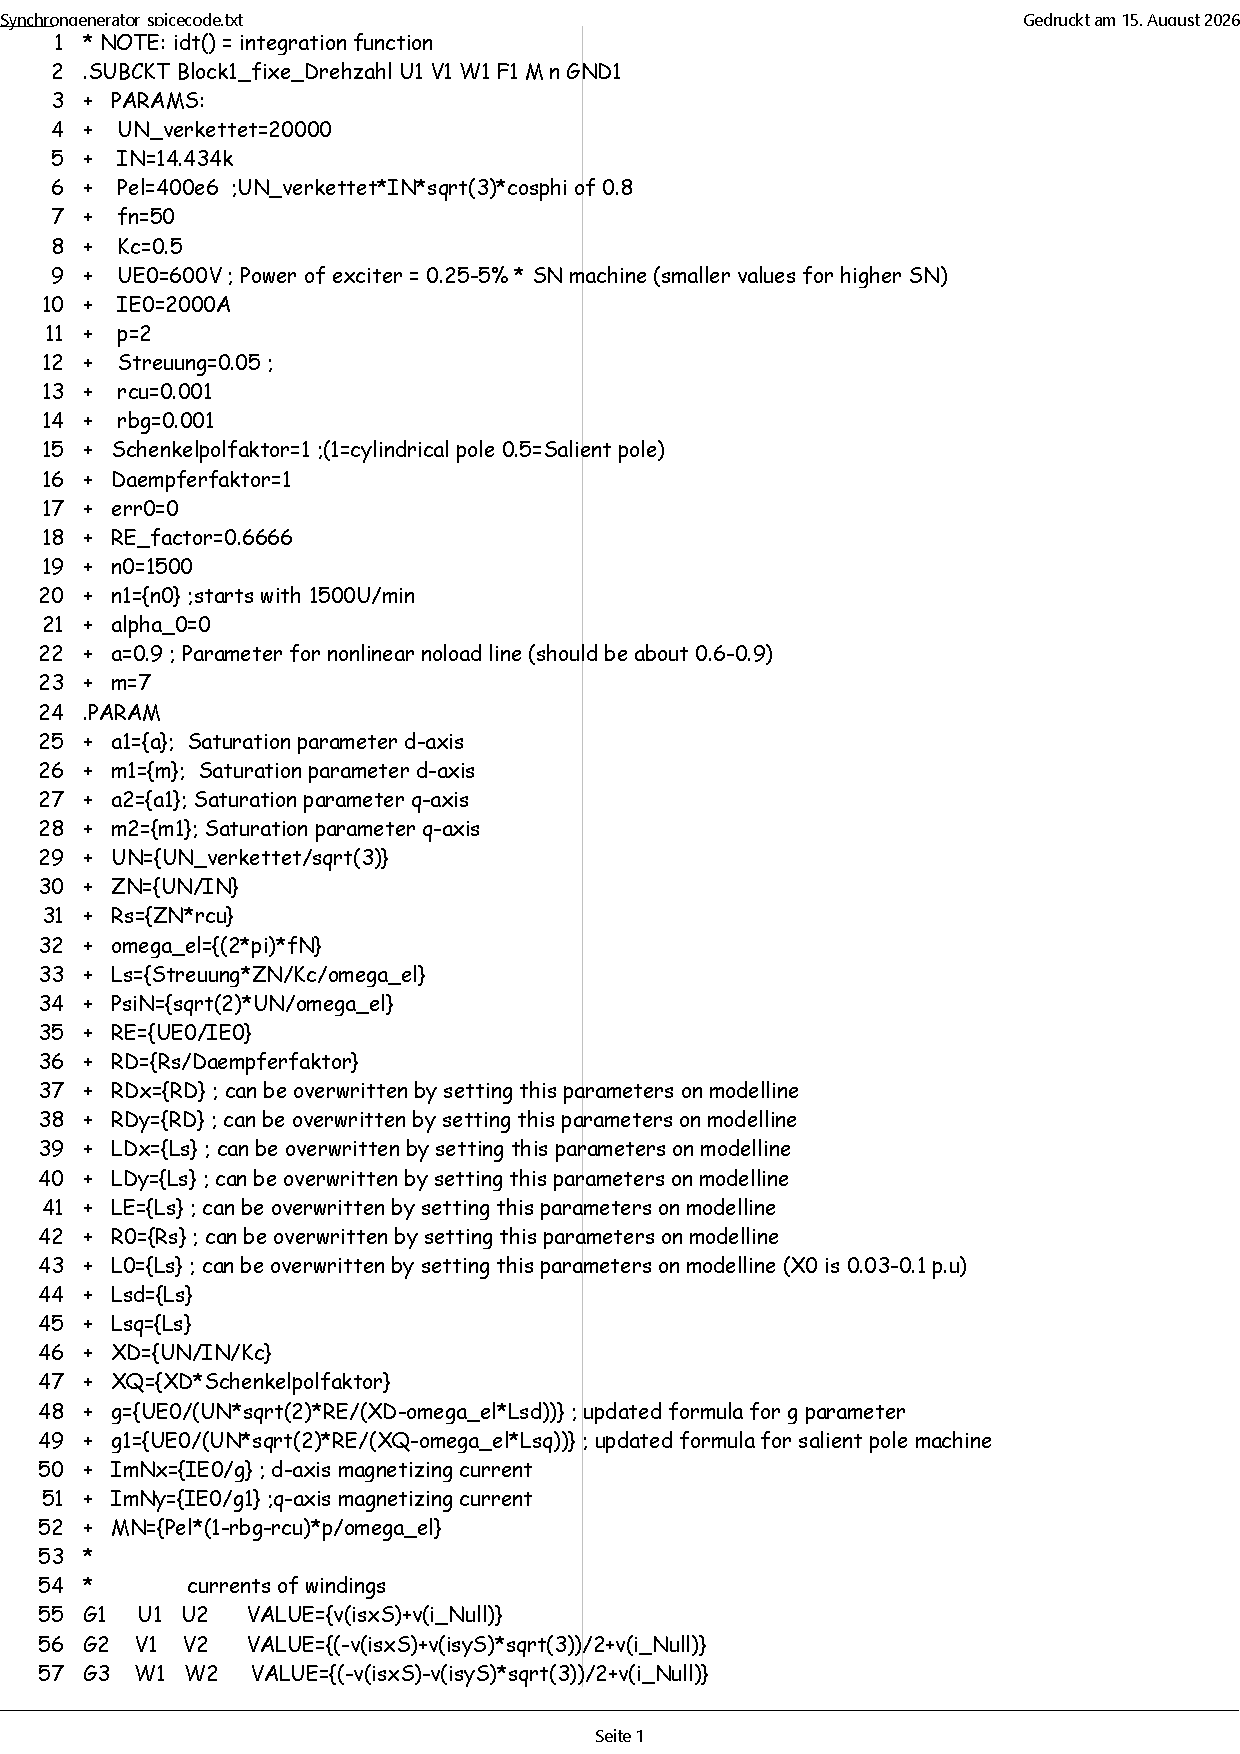
\includegraphics[width=0.90\textwidth]{figures/Synchronmaschine_SpiceCode_1.pdf}
%	\caption{Spice Listing for synchronous machine model page1 of 2}
%	\label{fig:Synchronous machine listing1}
%\end{figure}
%
%\begin{figure}[H]
%	\centering
%	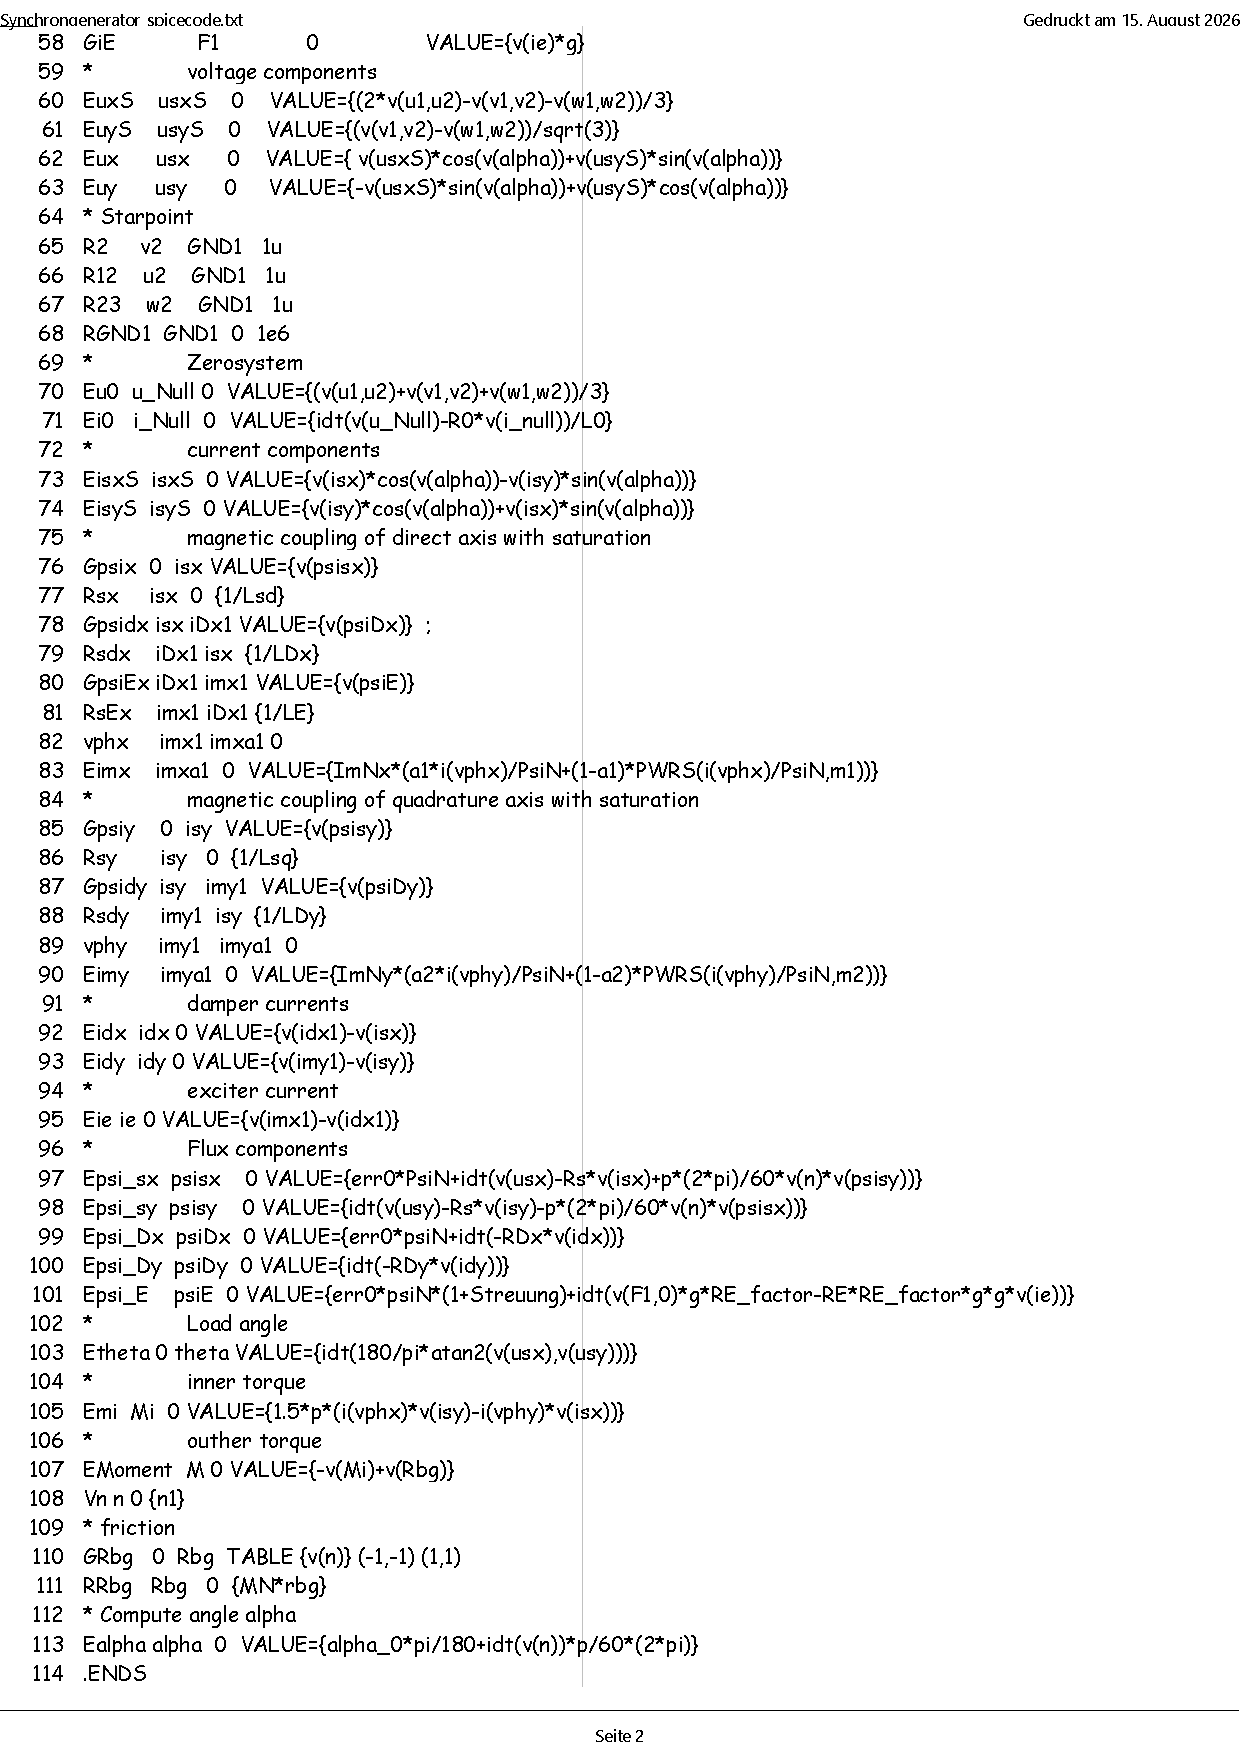
\includegraphics[width=0.90\textwidth]{figures/Synchronmaschine_SpiceCode_2.pdf}
%	\caption{Spice Listing for synchronous machine model page2 of 2}
%	\label{fig:Synchronous machine listing2}
%\end{figure}

\begin{figure}[H]
	\centering
	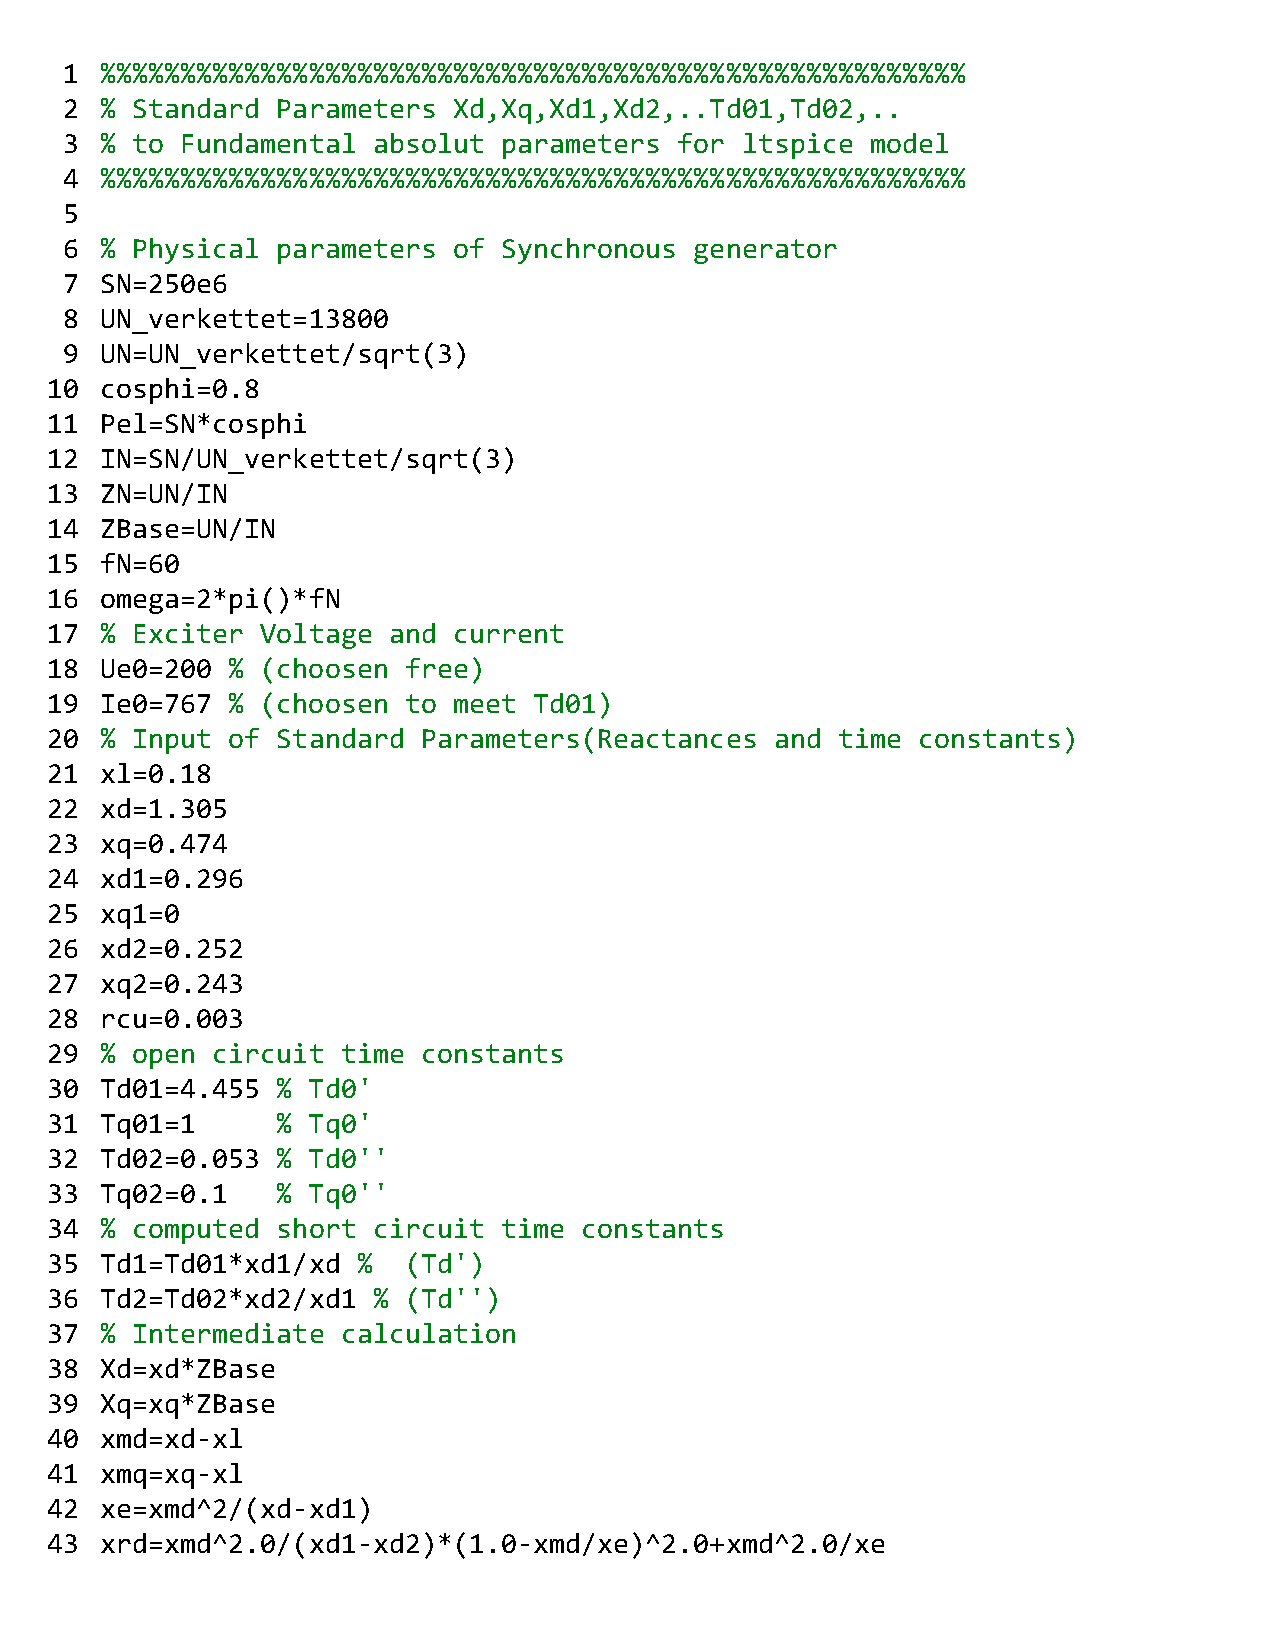
\includegraphics[width=0.90\textwidth]{figures/Matlab_Standardparameters_to_Fundamentalparameters 1.pdf}
	\caption{MATLAB code for converting standard machine parameters to fundamental model parameters}
	\label{fig:Standard to fundamental parameters}
\end{figure}

\begin{figure}[H]
	\centering
	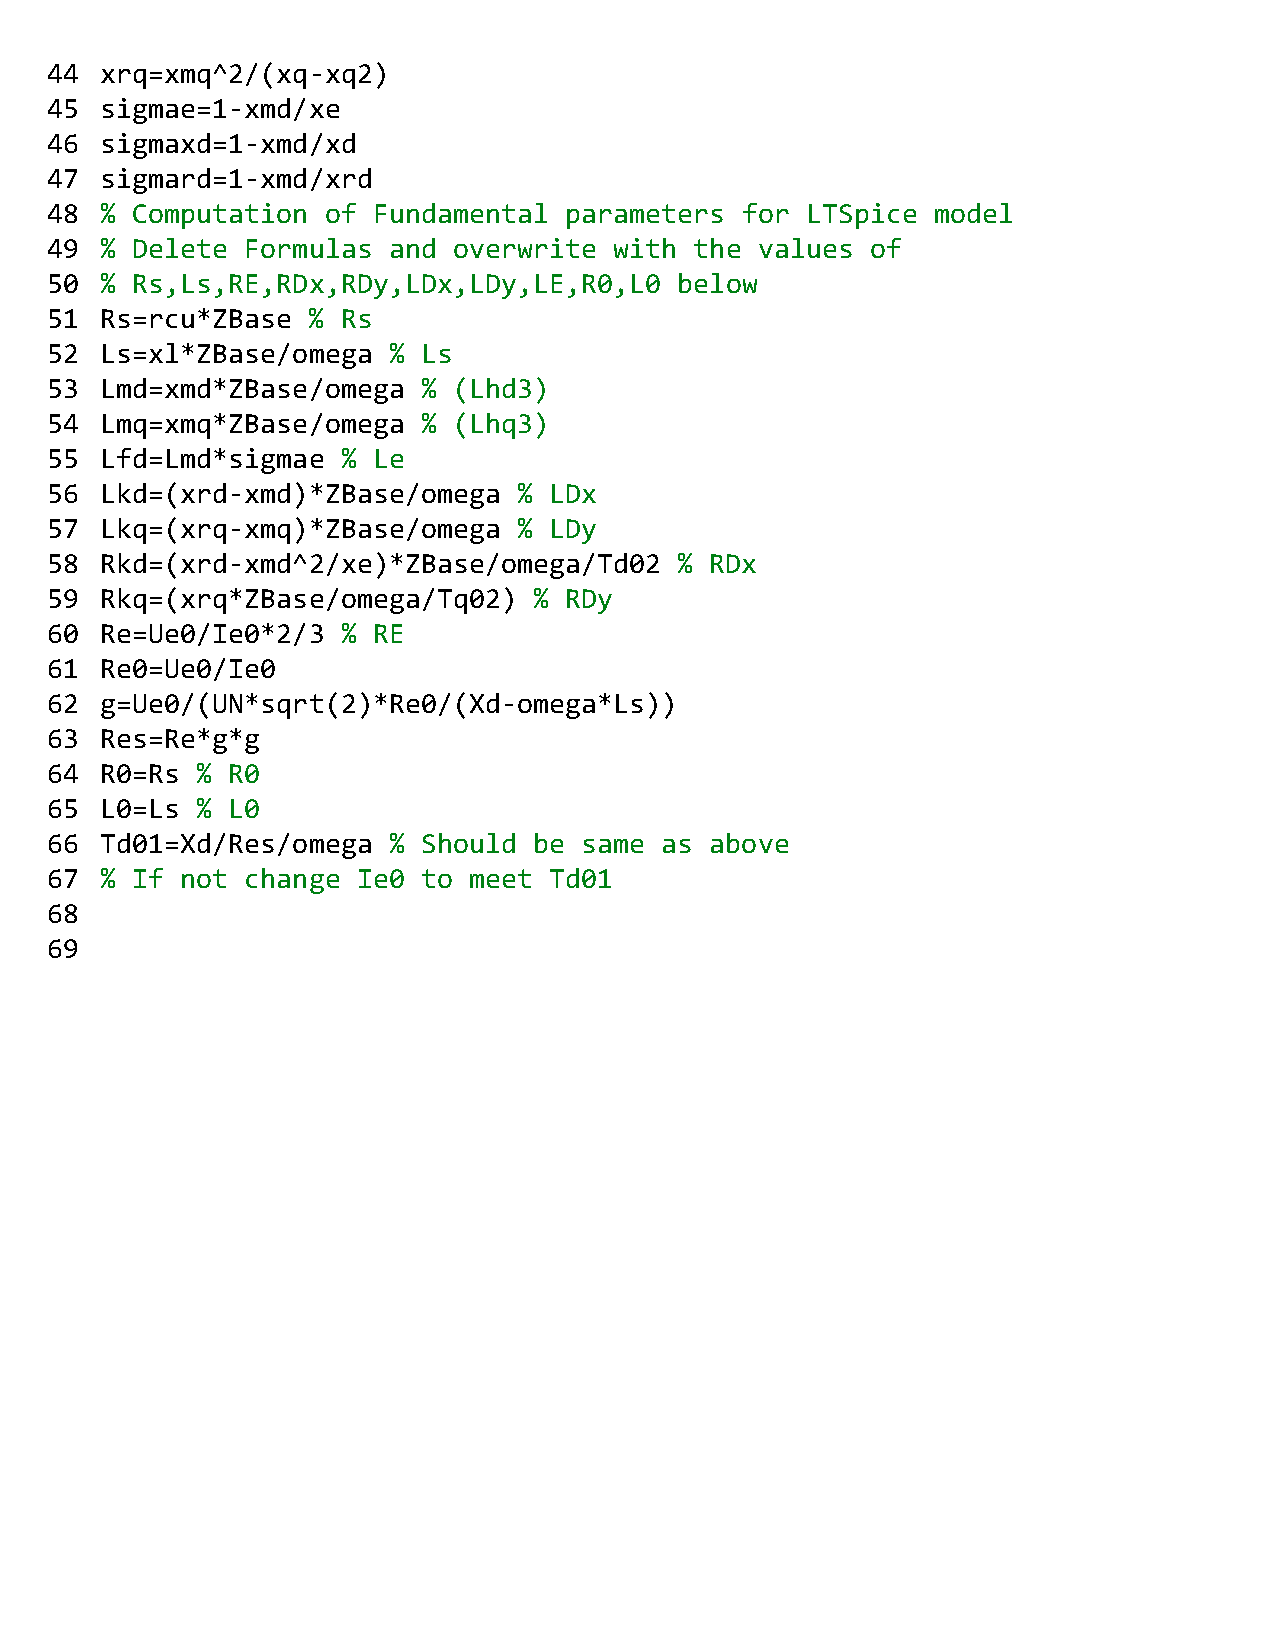
\includegraphics[width=0.90\textwidth]{figures/Matlab_Standardparameters_to_Fundamentalparameters 2.pdf}
	\caption{MATLAB code for converting standard machine parameters to fundamental model parameters}
	\label{fig:Standard to fundamental parameters}
\end{figure}	
		



